% Copyright (c) 2024 Alexander Bluhm <bluhm@genua.de>
%
% Permission to use, copy, modify, and distribute this software for any
% purpose with or without fee is hereby granted, provided that the above
% copyright notice and this permission notice appear in all copies.
%
% THE SOFTWARE IS PROVIDED "AS IS" AND THE AUTHOR DISCLAIMS ALL WARRANTIES
% WITH REGARD TO THIS SOFTWARE INCLUDING ALL IMPLIED WARRANTIES OF
% MERCHANTABILITY AND FITNESS. IN NO EVENT SHALL THE AUTHOR BE LIABLE FOR
% ANY SPECIAL, DIRECT, INDIRECT, OR CONSEQUENTIAL DAMAGES OR ANY DAMAGES
% WHATSOEVER RESULTING FROM LOSS OF USE, DATA OR PROFITS, WHETHER IN AN
% ACTION OF CONTRACT, NEGLIGENCE OR OTHER TORTIOUS ACTION, ARISING OUT OF
% OR IN CONNECTION WITH THE USE OR PERFORMANCE OF THIS SOFTWARE.

\documentclass[14pt]{beamer}
\usetheme{Frankfurt}
\usepackage{tikz}
\usepackage{graphicx}
\usepackage{varwidth}
\usepackage{tipa}
\usepackage{alltt}
\usepackage{xcolor}
\usepackage{upquote}
\usepackage[T1]{fontenc}
\usepackage{textcomp}
\usetikzlibrary{shapes.arrows}
\usetikzlibrary{shapes.geometric}
\usetikzlibrary{shapes.multipart}
\usetikzlibrary{shapes.symbols}
\author{Alexander Bluhm}
\title{A Packet's Journey Through the OpenBSD Network Stack}
\institute{genua GmbH\\ \url{bluhm@genua.de}\\ \url{bluhm@openbsd.org}}
\date{September 2024}
\let\Tiny\tiny

\begin{document}

\begin{frame}
\titlepage
\end{frame}

\begin{frame}{Agenda}
\setcounter{tocdepth}{1}
\tableofcontents
\end{frame}

\section{Overview}

\subsection{Environment}
\begin{frame}{Environment}
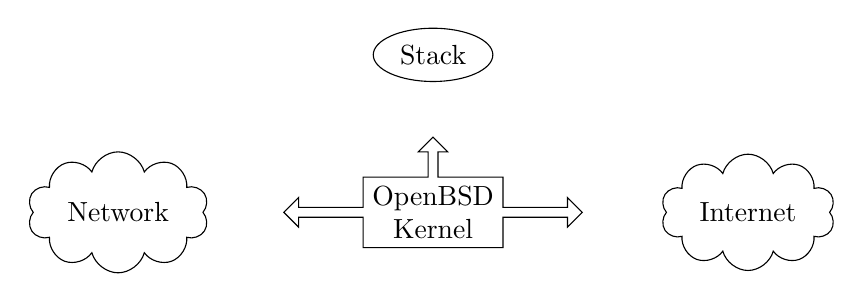
\begin{tikzpicture}
  \node [cloud, draw, aspect=2]
    at (-4, 0)
    {Network};
  \node [align=center, arrow box, draw,
    arrow box arrows={east:1cm, north:.5cm, west:1cm}]
    at (0, 0)
    {\begin{varwidth}{\textwidth}\centering OpenBSD \\ Kernel\end{varwidth}};
  \node [cloud, draw, aspect=2]
    at (4, 0)
    {Internet};
  \node [ellipse, draw, aspect=2]
    at (0, 2)
    {Stack};
\end{tikzpicture}
\end{frame}

\subsection{Layer}
\begin{frame}{Layer}
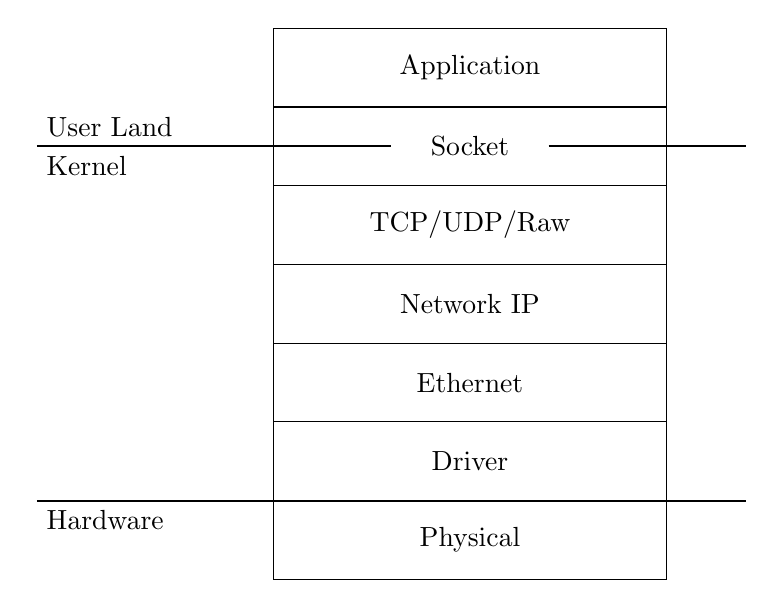
\begin{tikzpicture}
  \draw (-1,0) rectangle +(5,1) node(l1) [midway] {Physical};
  \draw (-1,1) rectangle +(5,1) node(l1) [midway] {Driver};
  \draw (-1,2) rectangle +(5,1) node(l2) [midway] {Ethernet};
  \draw (-1,3) rectangle +(5,1) node(l3) [midway] {Network IP};
  \draw (-1,4) rectangle +(5,1) node(l4) [midway] {TCP/UDP/Raw};
  \draw (-1,5) rectangle +(5,1) node(l5) [midway] {Socket};
  \draw (-1,6) rectangle +(5,1) node(l5) [midway] {Application};
  \draw[thick] (-4,5.5) node(context) {} -- +(4.5,0) +(6.5,0) -- +(9,0);
  \node [below right] at (context) {Kernel};
  \node [above right] at (context) {User Land};
  \draw[thick] (-4,1) node(hardware) {} -- +(9,0);
  \node [below right] at (hardware) {Hardware};
\end{tikzpicture}
\end{frame}

\subsection{Flow}

\subsection{Data}

\section{Conclusion}

\subsection{Links}
\begin{frame}{Links}
\begin{itemize}
    \item these slides
	{\small \url{https://github.com/bluhm/talk-packetflow}}
\end{itemize}
\end{frame}

\subsection{Questions}
\begin{frame}{Questions}
\begin{center}
\begin{tikzpicture}
\draw [font=\Huge] node {?};
\end{tikzpicture}
\end{center}
\end{frame}

\end{document}
